\documentclass{beamer}
\DeclareFontShape{OT1}{cmss}{b}{n}{<->ssub * cmss/bx/n}{} 
\usetheme{default}
\usepackage{amsmath}
\usepackage{amsfonts}
\usepackage{mathbbol}
\usepackage{xcolor} % before tikz or tkz-euclide if necessary
\usepackage{tkz-euclide} % no need to load TikZ
\usepackage{multirow}
\usepackage{lmodern}
\usepackage{bm}
\usepackage{subcaption}
%\usepackage{subfigure}

\usepackage[
backend=biber,
style=authoryear-icomp,
sortlocale=de_DE,
natbib=true,
url=false, 
doi=true,
eprint=false
]{biblatex}
\addbibresource{../Bibliography/main_ML.bib}



\titlegraphic{
\includegraphics[width=2cm]{../Figures/UAMS_RGB.png}
}


\title{Neuroinformatics Journal Club\\ Dynamic Brain Networks (HMM)}
\author{Horacio G\'omez-Acevedo\\ Department of Biomedical Informatics\\
	University of Arkansas for Medical Sciences}

\begin{document}
	\begin{frame}[plain]
		\maketitle
	\end{frame}
	
\begin{frame}{Today's paper}
	\begin{figure}[h]
	\centering
%	\begin{subfigure}{0.4\textwidth}
%		\centering
		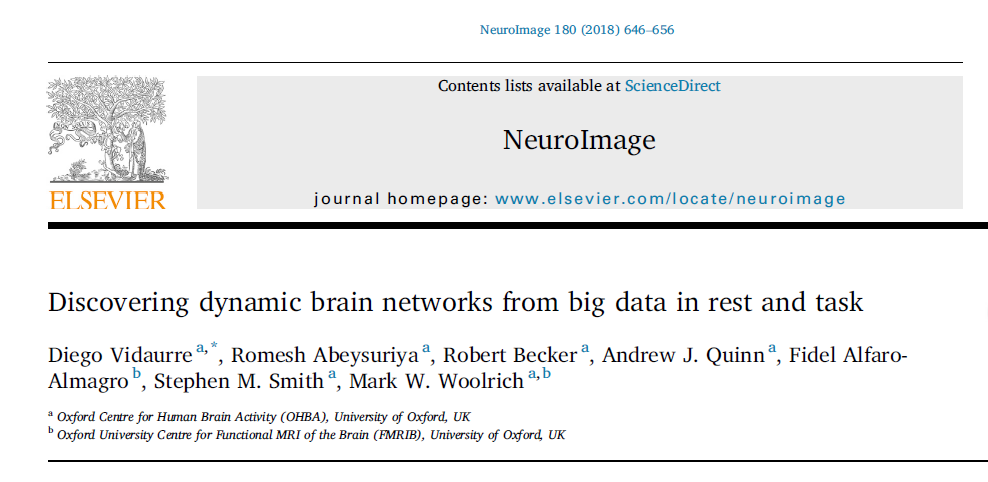
\includegraphics[scale=0.6]{../Figures/vidaurre_paper.png}
%	\end{subfigure}
	\end{figure}
\end{frame}

\begin{frame}{Journal Club Format}
	This is a new format for Journal Club
	\begin{itemize}
		\item We will explore more carefully the methodology.
		\item Most of the papers are going to require "heavy" tools from computer sciences, statistics and mathematics. 
		\item It will be a transition time to understand each other (be patient)
		\item The dynamical nature of brain activity will make it very challenging to hold on to a single model. 
		\item Complexity vs. Explainability is an implicit trade-off. 
		\item The ultimate goal is to use and expand "acceptable" methodologies into new and more "appropriate" ones. Yes, this means \textbf{coding} (R, Python, MatLab).
	\end{itemize} 
\end{frame}

\begin{frame}{Hidden Markov Models}
	The implementation of Hidden Markov models dates back in the late 60's by Leonard Baum and collaborators. It is still an active area of research. 	
	
	What is a Markov chain?
	\begin{figure}[h]
		\centering
		%	\begin{subfigure}{0.4\textwidth}
			%		\centering
			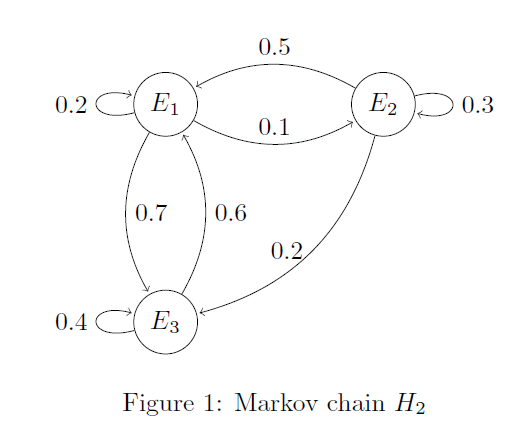
\includegraphics[scale=0.6]{../Figures/fig_markov_chain.png}
			%	\end{subfigure}
	\end{figure}
	
	
\end{frame}

\begin{frame}{Hidden Markov Chains}
	The fair casino problem 
	\begin{itemize}
		\item You don't know if the dealer has a fair or unfair coin (Hidden states)
		\item You only observe the output (Emissions)
	\end{itemize}
		\begin{figure}[h]
		\centering
		%	\begin{subfigure}{0.4\textwidth}
			%		\centering
			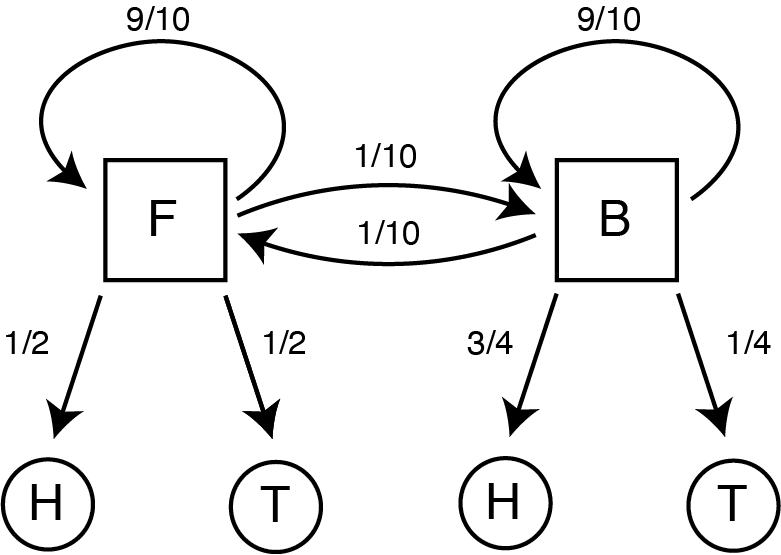
\includegraphics[scale=0.6]{../Figures/hmm_fair_casino.png}
			%	\end{subfigure}
	\end{figure}
\end{frame}

\begin{frame}{Hidden Markov Chains (Genomics)}
	Another (unrealistic) example is to build a HMM to describe a (genetic) sequence
	
	\begin{figure}[h]
	\centering
	%	\begin{subfigure}{0.4\textwidth}
		%		\centering
		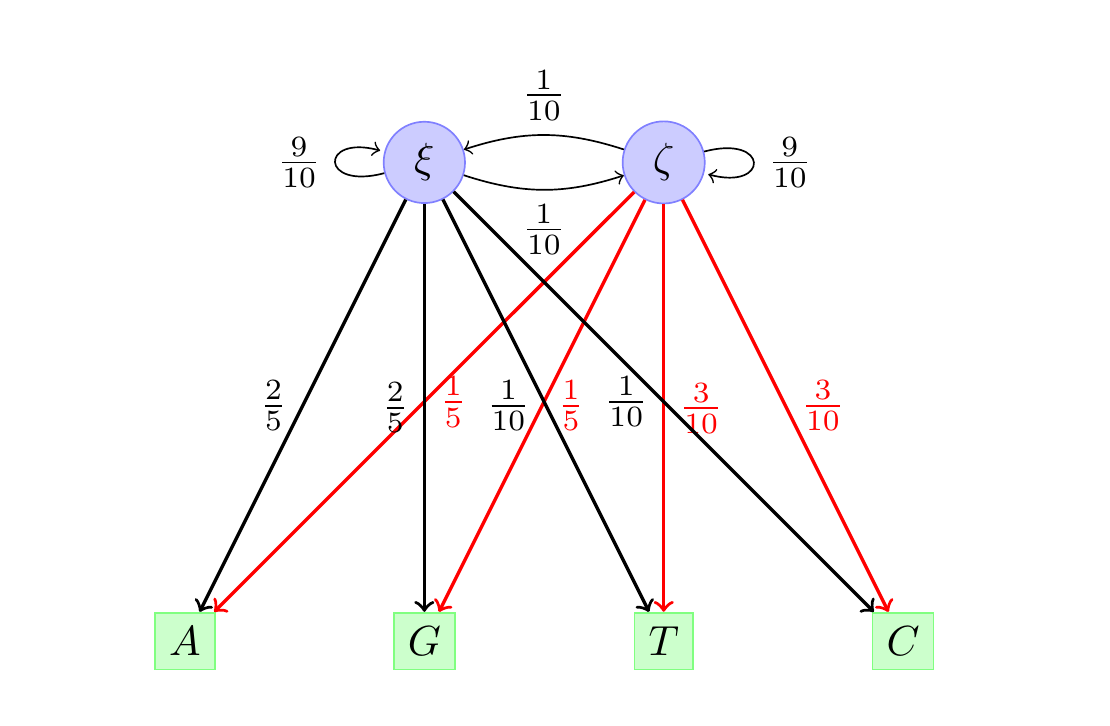
\includegraphics[scale=0.5]{../Figures/hmm_example.png}
		%	\end{subfigure}
\end{figure}
\end{frame}
\begin{frame}{Viterbi's representation HMMs}
		\begin{figure}[h]
		\centering
		%	\begin{subfigure}{0.4\textwidth}
			%		\centering
			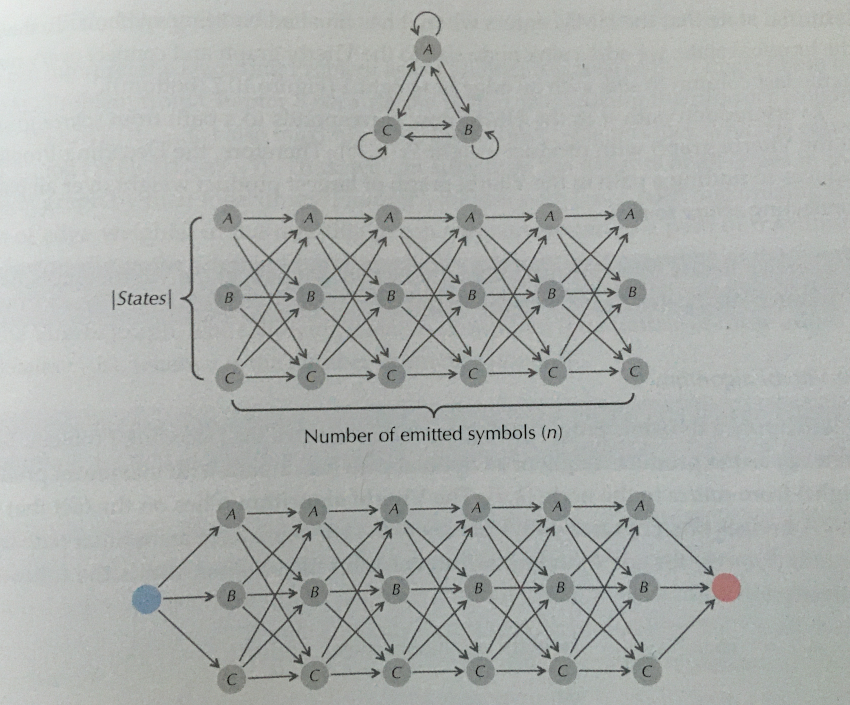
\includegraphics[scale=0.6]{../Figures/fig_hmm.png}
			%	\end{subfigure}
	\end{figure}
\end{frame}

\begin{frame}{Building a HMM}
	From Baker et al. 2014
\begin{quote}	
Here, we present a study that identifies transient networks of brain activity, with no prior assumptions
on the brain areas or time scales involved. This uses a distinct methodology based on a hidden
Markov model (HMM), which infers a number of discrete brain states that recur at different points in
time. Each inferred state corresponds to a unique pattern of whole-brain spontaneous activity, which
is modeled by a multivariate normal distribution and a state time course indicating the points in time
at which that state is active. These two outputs are shown schematically in Figure 1, and allow us to
describe both the spatial and temporal characteristics of each inferred state.
\end{quote}
\end{frame}

\begin{frame}{Building a HMM}
		\begin{figure}[h]
			\centering
			%	\begin{subfigure}{0.4\textwidth}
				%		\centering
				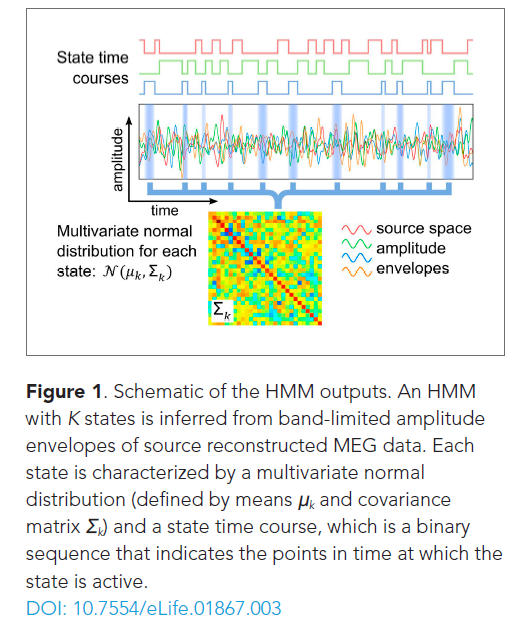
\includegraphics[scale=0.6]{../Figures/fig_hmm_baker.png}
				%	\end{subfigure}
		\end{figure}
\end{frame}

\begin{frame}{In the paper}
	
\begin{quote}
	The HMM is a family of models that can describe time series of data
	using a discrete number of states, all having the same probabilistic distributions
	but each having different distribution parameters. Thus, the
	states correspond to unique patterns of brain activity that recur in
	different parts of the time series. For each time point t, a state variable
	dictates the probability of each state being active at that moment
\end{quote}
\end{frame}

\begin{frame}{General HMM at rest}
			\begin{figure}[h]
		\centering
		%	\begin{subfigure}{0.4\textwidth}
			%		\centering
			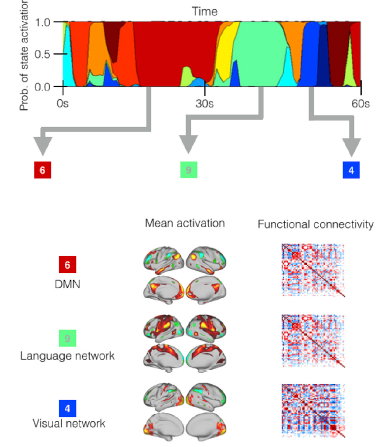
\includegraphics[scale=0.6]{../Figures/fig_vidaurre_1a.png}
			%	\end{subfigure}
	\end{figure}
\end{frame}

\begin{frame}{General HMM in task}
	\begin{figure}[h]
		\centering
		%	\begin{subfigure}{0.4\textwidth}
			%		\centering
			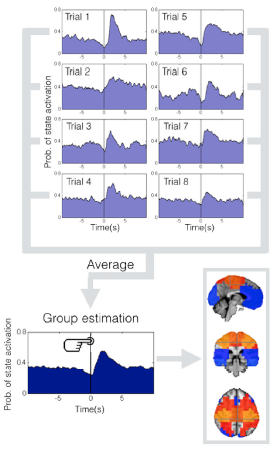
\includegraphics[scale=0.6]{../Figures/fig_vidaurre_1b.png}
			%	\end{subfigure}
	\end{figure}
\end{frame}

\begin{frame}{General HMM cont }
\begin{quote}
	an HMM
	generally comprises the description of the states, the state time courses
	(which determines the probability of each state to be active at each time
	point in the time series) and the transition probabilities between the
	states (i.e. the probability to transition from each state to each other
	state). Because here we run the HMM on all concatenated subjects'
	datasets, the states and the transition probabilities are defined at the
	group level; the state time courses are however particular to each subject
	- that is, states can come active at different moments for each subject.
	Since the probability distribution of each part of the model depends on all
	others, there is no closed-form solution available
\end{quote}
\end{frame}
%\begin{frame}{References}
%	Materials and some of the pictures are from \citep{calin}.
%	\printbibliography 	
	
%	I have used some of the graphs by hacking TiKz code from StakExchange, Inkscape for more aesthetic plots and other old tricks of \TeX
	
%\end{frame}


\end{document}
